
\documentclass[11pt, a4paper, german]{article}
\usepackage[utf8]{inputenc}
\usepackage{amsmath}
\usepackage{amsfonts}
\usepackage{amssymb}
\usepackage{algorithm}
\usepackage{algorithmic}
\usepackage{makeidx}
\usepackage{graphicx}
\usepackage{tabularx}
\usepackage{bbm}
\usepackage[ngerman]{babel}
\usepackage{BA_Titelseite}
\usepackage[colorlinks=false, pdfborder={0 0 0}]{hyperref}
\bibliographystyle{unsrt}

%Namen des Verfassers der Arbeit
\authornew{Boris Prochnau}

%Geburtsdatum des Verfassers
\geburtsdatum{22. Dezember 1989}
%Gebortsort des Verfassers
\geburtsort{Tartu}
%Datum der Abgabe der Arbeit
\date{\today}

%Name des Betreuers
% z.B.: Prof. Dr. Peter Koepke
\betreuer{Betreuer: Prof. Dr. Anton Bovier}
%Name des Instituts an dem der Betreuer der Arbeit tätig ist.
%z.B.: Mathematisches Institut
\institut{Institut für Angewandte Mathematik}
%Titel der Bachelorarbeit
\title{Simulation normalisierter BPDL Prozesse}
%Do not change!
\ausarbeitungstyp{Bachelorarbeit Mathematik}



\begin{document}

\maketitle
\tableofcontents

\clearpage


\section{Einleitung}
Das Ziel dieser Bachelorarbeit ist es eine Programm zu entwickeln welches den zeitlichen Verlauf von sogenannten normalisierten BPDL Prozessen graphisch darstellt.\\
Diese BPDL (von Bolker, Pacala, Dieckmann und Law) Prozesse basieren auf einem stochastischen Populationsmodell, welches im n"achsten Kapitel n"aher vorgestellt wird. \\

Dem Programm sollte es m"oglich sein die Parameter einer Population festlegen zu k"onnen und die Entwicklung dieser Population schlie"slich zeitlich verfolgen zu k"onnen. Auf diese Weise soll man beobachten k"onnen ob sich ein Merkmal gegen"uber einem anderen Durchsetzten kann oder sich ein stabiler Zustand einpendelt. Insbesondere kann der Einfluss der Normalisierung auf das vorzeitige Aussterben eines Prozesses deutlich dargestellt werden.\\

Alle Simulationen basieren auf einem Modell, dass jedes Lebewesen einer Population (z.B. Pflanzen) ein bestimmtes Merkmal tr"agt. Diese Merkmale werden durch Wettbewerb zu jeder existenten Gruppe, Geburten und Todesraten klassifiziert. Schlie"slich ist es jedoch die Entwicklung der Population und nicht der Individuen die simuliert werden soll, weshalb man im simulierten Prozess zwar den Tod und die Geburt von Individuen verfolgen kann, aber nicht die Entwicklung spezieller Individuen. Der "Ubergang zu dieser Sichtweise wird n"aher im 2. Kapitel beschrieben und kr"ont in der Konvergenz zu einer deterministischen Funktion.\\

Um zu Pr"ufen ob und wie schnell der Prozess gegen seinen Stabilen Zustand konvergiert, werden in der Simulation auch stabile Zust"ande f"ur diverse Situationen automatisch dazu gestellt. Anhand dieser k"onnen individuelle und dynamische Abbruchkriterien formuliert werden.\\

Schlie"slich werde ich noch kurz die TSS Prozesse und ein weiteres Programm vorstellen, welches die bisher betrachteten BPDL Prozesse erweitert auf TSS-Prozesse. Dabei sollen nicht nur das besonders interessante Verhalten vom Wechsel des dominanten Merkmals simuliert werden, sondern es wird eine verbesserte Laufzeit durch Interpolation vorgestellt die eine effiziente Simulation trotz sehr gro"ser Zeit und besonders pr"azise Betrachtung von Aktionsreichen Gebieten anbietet.


%Dabei ist das Interesse besonders bei normalisierten BPDL Prozessen und schließlich auch bei TSS (trait subsitution sequence) Prozessen.\\
%Dabei reicht es nicht einfach eine Implementierung zu machen, denn durch die Zufallseigenschaft lässt sich nicht so einfach die Korrektheit verifizieren. Gerade bei TSS Prozessen ist die Anzahl der Mutationen und deren Abstände und Invasionschancen entscheidend.\\
%Zu diesem Zweck wird ein Teil der Arbeit diese Problemstellung behandeln.

\clearpage
\section{Modell}
Das verwendete Model lehnt sich an das Model aus \cite{Champagnat20061127} an. Dieses nutzt die drei grundlegenden Mechanismen von Darwins Evolutionslehre: Vererbung, Variation (Mutationen) und Selektion durch Wettbewerb um eine Menge von Merkmalen f"ur Individuen zu beschreiben. Diese bestimmen die F"ahigkeit des Individuums zu "uberleben und sich fortzupflanzen.\\
Jedoch wurden für meine Simulation einige kleine Änderungen gewünscht die im Anschluss erl"autert werden. \\
	\subsection{Grundlagen}
	Sei $ X $ der Raum der Merkmale. Jedes Individuum hat genau ein solches Merkmal $ x \in X $. Der Einfachheit halber sei X eine Indexmenge: $ X = \{1,\dots, n\} $ repräsentativ für eine Durchzählung der Merkmale und im folgenden seien $ x,y \in X $ zwei solche Merkmale. Au"serdem gilt:
	\begin{itemize}
		\item Jedes Individuum kann sich asexuell fortpflanzen oder sterben.
		\item Fortpflanzungs- und Todeszeitpunkte k"onnen durch sogenannte exponentielle Uhren (wie in \cite[S. 3]{fournier2004microscopic}) beschrieben werden. Diese Uhren haben exponentiell verteilte Weckzeiten. Durch die Gedächtnislosigkeit der Exponentialverteilung, können alle Uhren nach dem ersten Klingeln neu gestellt werden. 
		\item Die Fortpflanzung eines Individuums aus $ x $ kann jedoch auch in der Geburt eines Individuums in $ y $ resultieren.
	\end{itemize}
	Sp"ater wird deutlich dass die Zur"uckstellbarkeit der Uhren entscheiden ist um die Sichtweise von der Ebene des Individuums auf die der gesamten Population zu heben.\\
	Diese Todes und Fortpflanzungs- Ereignisse eines Individuums haben feste Raten die das dazugeh"orige Merkmal beschreiben.\\
	
	\begin{tabular}{r p{26em}}
		$ b(x) $: & Ist die Geburtenraten durch ein Individuum mit Merkmal $ x $.\\
		$ d(x) $: & Ist die natürliche Todesrate.\\
		$ c(x, y) $: & Ist die Todesrate durch Wettbewerb zwischen Individuen mit Merkmal x und y.\\
		$ \mu $: & Ist die Mutationswahrscheinlichkeit "{}auf die Nachbarn"{} mit je $ \frac{\mu}{2} $ pro Nachbar. \\
	\end{tabular}\\

	Schlie"slich lassen sich durch Superposition z.B. die beiden Todesraten zu einer gemeinsamen Todesrate zusammenfassen oder die arteigene Geburtenrate abtrennen.\\
	
	\begin{tabular}{ r p{18em} }
		$ b(x) \cdot (1 - \mu) $: & ist die arteigene Geburtenrate eines Individuums mit Merkmal $ x $\\
		$ d(x) + \sum_{i=1}^{N_t} c(x, x_i) $: & ist die gesamte Todesrate eines Individuums mit Merkmal x (mit $ N_t := $ \#Individuen zur Zeit t mit Merkmal $ x $ und $ x_i $ das Merkmal des i-ten Individuums).\\
		$ d(x) + \sum_{y=1}^{n} c(x,y) \cdot n_t(x) $: & wie oben, nur mit $ n := $ \#Merkmale, und $ n_t(x) :=$ \#Individuen zur Zeit t mit Merkmal $ x $
	\end{tabular}\\
	
	Die letzte Darstellung der Todesrate ist praktischer f"ur die Betrachtung der Population. "Ahnlich k"onnen weitere Ereignisse zusammengefasst werden, so dass man z.B. eine Todesrate und eine arteigene Geburtenraten der Merkmale erstellen kann:

	\begin{itemize}
	 	\item Arteigene Geburtenrate des Merkmals $ x $: 
	 	\[ b(x) \cdot (1 - \mu) + \left( b(x+1) \cdot \mathbbm{1}_{x<n} + b(x-1) \cdot \mathbbm{1}_{x>1} \right) \cdot \frac{\mu}{2} \] 
	 	\item Gesamte Todesrate des Merkmals $ x $: 
	 	\[ d(x) + \sum_{y=1}^{n} c(x,y) \cdot n_t(y) \]
	\end{itemize}
	
	Die Simulation soll die Entwicklung der Merkmale und nicht die Ereignisse der Individuen darstellen, daher ist es unpraktisch weiterhin die Raten jedes Individuums zu berechnen. Alternativ k"onnen Ereignisse zu denen von Merkmalen zusammengefasst werden:
	\begin{itemize}
		\item Fortpflanzungsrate des Merkmals $ x $: 
		\[ B_1(x) = b(x) \cdot n_t(x) \]
		\item Oder alternativ die Geburtenrate (Wachstumsrate) des Merkmals $ x $: 
		\begin{align*}
			B_2(x)  & = (1 - \mu) \cdot b(x) \cdot n_t(x)\\
				  & + \frac{\mu}{2} \cdot b(x+1) \cdot n_t(x+1) \cdot \mathbbm{1}_{x<1}\\
				  & + \frac{\mu}{2} \cdot b(x-1) \cdot n_t(x-1) \cdot \mathbbm{1}_{x>1}
		\end{align*}
		\item Todesrate des Merkmals $ x $: 
		\[ D(x) = d(x) \cdot n_t(x) + n_t(x) \cdot \sum_{y=1}^{n} c(x,y) \cdot n_t(y) \]
	\end{itemize}
	Das entspricht 2 wesentlichen exponentiellen Uhren pro Merkmal. Eine für Tod und eine für Geburt innerhalb des Merkmals.\\
	F"ur die Simulation ist eine Gesamtrate für das Eintreten eines Ereignisses praktischer. Auf diese Weise wird nur auf das Eintreffen einer Uhr gewartet.
	\begin{itemize}
		\item Ereignisrate des Merkmals $ x $ (Trait Rate):
		\[ TR(x) = B(x) + D(x) \]
		\item Totale Ereignis Rate (Total Event Rate): 
		\[ TER = \sum_{x \in X} TR(x)\]
	\end{itemize}
	Mit der Totalen Ereignisrate gibt es jetzt eine Rate die es erlaubt eine Zufallsvariable für das Eintreffen einer Variable zu ziehen. Anschließend ist es nur noch erforderlich (mit der Ziehung zwei weiterer Zufallsvairablen) festzustellen welchem Merkmal welches Ereignis zukommt. Das Zusammenfassen der Raten vereinfacht es dem Programm sp"atere Auswertungen und Funktionen Bereit zu stellen. So l"asst sich z.B. aus der Geburtenrate (Wachstumsrate) eines ausgestorbenen Merkmals die Mutationsrate ablesen, ohne weitere Berechnungen machen zu m"ussen.\\
	
	\subsection{BPDL Prozess}
	Die Population wird durch die Zufallsvariable
	\[ \nu_t = \sum_{i=1}^{N_t} \delta_{x_i} \]
	beschrieben. \\
	Damit ist $ \nu_t $	ein stochastischer Prozess, genauer ein Markov Sprung Prozess auf dem Raum:
	\[ \nu_t \in M_F(X) = \left\{ \sum_{i=1}^{n} \delta_{x_i}, n \in \mathbb{N}, x_1, \dots, x_n \in X \right\} \]
	Man erkennt leicht die Sprungeigenschaft:
	\[ \int_X 1 \text{ } \nu_t(dx) = N_t 
	\text{ und }
	\int_X \mathbbm{1}_y(x) \text{ } \nu_t(dx) = n_t^{y} \]
	Normalerweise geh"ort zum Model des BPDL Prozesses, dass die Mutationen auf einem beliebigen Merkmal (nicht nur den Nachbarn) landen k"onnen. F"ur einen solchen Prozess ist der Generator definiert als:
	\begin{align*}
		L_{\phi(\nu)} &= \int_{X} b(x)(1-\mu)[\phi(\nu + \delta_x) - \phi(\nu)]\nu(dx)\\
					  &+ \int_{X}\int_{\mathbb{R}^d} b(x) \cdot \mu [\phi(\nu + \delta_{x+z}) - \phi(\nu)] m(x,dz) \nu(dx)\\
				  	  &+ \int_{X} d(x)[\phi(\nu - \delta_x) - \phi(\nu)]\nu(dx)\\
				 	  &+ \int_{X} \left( \int_{X} c(x,y) \nu(dy) \right) [\phi(\nu - \delta_x) - \phi(\nu)]\nu(dx)
	\end{align*}
	mit $ \phi: M_F \to \mathbb{R} $\\
	Der f"ur unser Model angepasster Generator m"usste folgende Form haben:
	\begin{align*}
		L_{\phi(\nu)} &= \int_{X} b(x)(1-\mu)[\phi(\nu + \delta_x) - \phi(\nu)]\nu(dx)\\
					  &+ \int_{X} b(x) \cdot \mu \cdot \mathbbm{1}_{x > 0} 
					  [\phi(\nu + \delta_{x-1}) - \phi(\nu)]  \nu(dx)\\
					  &+ \int_{X} b(x) \cdot \mu \cdot \mathbbm{1}_{x < n} 
					  [\phi(\nu + \delta_{x-1}) - \phi(\nu)]  \nu(dx)\\
					  &+ \int_{X} d(x)[\phi(\nu - \delta_x) - \phi(\nu)]\nu(dx)\\
					  &+ \int_{X} \left( \int_{X} c(x,y) \nu(dy) \right) [\phi(\nu - \delta_x) - \phi(\nu)]\nu(dx)
	\end{align*}
	mit $ \phi: M_F \to \mathbb{R} $\\	

		
		
	
	
\clearpage
\section{Normalisierung und Eigenschaften des BPDL Prozesses}

\subsection{Normalisierung des BPDL Prozesses}
	Wie schon zuvor erwähnt ist es für uns wichtig die Tode und Geburten nicht auf der Ebene des Individuums, sondern der gesamten Population zu betrachten. Dazu wird die LPA(Large Population Approximation) Normalisierung eingeführt.\\
	Dafür wird der Prozess mit einem Parameter K skaliert und es ergibt sich eine neue Zufallsvariable:
	\[ \nu_t^K := \frac{1}{K} \nu_t \]
	Um f"ur $ \nu_t^K $ das selbe Verhalten wie f"ur $ \nu_t $ zu erhalten, m"ussen einige Anpassungen vorgenommen werden.\\
	Zun"achst wird die Anfangsgröße $ n_0^K $ der Population proportional zu K gewählt.
	Die Raten für Geburten und natürliche Tode der Individuen bleiben unverändert. Da die Populationsgröße jedoch quadratisch in Wettbewerbsrate einfließt, sollte $ c^K = \frac{c}{K} $ gelten, da sonst wegen der hohen Population ein intensives Aussterben den Vergleich verf"alschen w"urde. Ein Beispiel dafür sieht folgendermaßen aus:
	\begin{figure}[H]
		\centering
		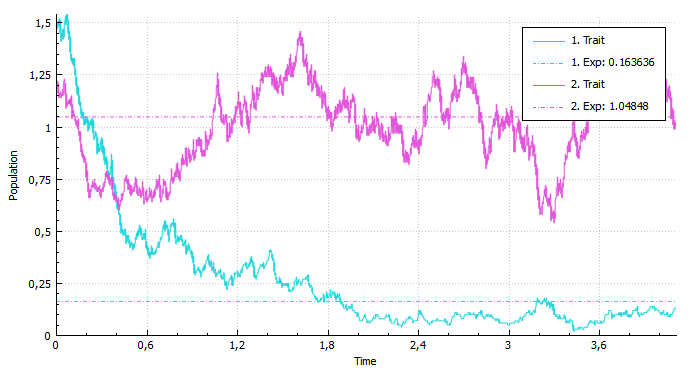
\includegraphics[width=0.7\linewidth]{./Pictures/LPANormalisierungK100}
		\caption[LPAK100]{LPA Normalisierung mit K=100}
		\label{LPA Normalisierung K=100}
	\end{figure}
	\begin{figure}[H]
		\centering
		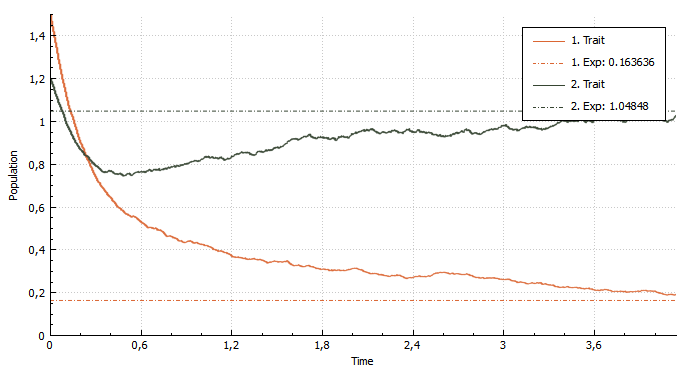
\includegraphics[width=0.7\linewidth]{./Pictures/LPANormalisierungK10000}
		\caption[LPAK100]{LPA Normalisierung mit K=10000}
		\label{LPA Normalisierung K=10000}
	\end{figure}
	
	\subsection{Fitness}
	
	\subsection{Equilibrium}
	Man erkennt dass die Merkmale für $ K \to \infty $ eine Konvergenz gegen eine Funktion $ \xi_t = n_t \delta_x $ aufweist. Diese Funktion wiederum konvergiert gegen einen stabilen Zustand (im folgenden Equilibrium genannt), worin sich die Populationsgröße nicht mehr ändert. Diese sehen für monomorphe und dimorphe Populationen ohne Mutation folgendermaßen aus:
	\begin{itemize}
		\item Monomorpher Population:\\
			\begin{align*}
			0 & = \dot{n} = (b(x) - d(x) - \bar{n}c(x,x))\bar{n}\\
			\bar{n}_x &= \frac{\left[ b(x)-d(x) \right]_+}{c(x,x)}
			\end{align*}
		\item Dimorphe Population:\\
			Auf die selbe Weise l"asst sich ein dimorpher stabiler Zustand ermitteln:
			\[ n_x = \frac{(b(x) - d(x))c(y,y)-(b(y)-d(y))c(x,y)}{c(y,y)c(x,x) - c(y,x)c(x,y)} \]
			\[ n_y = \frac{(b(y) - d(y))c(x,x)-(b(x)-d(x))c(y,x)}{c(y,y)c(x,x) - c(y,x)c(x,y)} \]
			Also sind $ (n_x, n_y) $, $ (\bar{n}_x, 0)$, $ (0, \bar{n}_y)$ oder $ (0,0) $ m"ogliche stabile Zust"ande im dimorphen Fall.
	\end{itemize}
	Die BPDL Simulationen erkennen dimorphe und monomorphe Populationen und stellen stets einen passenden stabilen Zustand $ n_x $, bzw. $ bar{n}_x $ dar. Um zu entscheiden unter welchen Voraussetzungen welcher stabile Zustand erreicht wird der folgende Satz helfen:


\clearpage

\noindent\rule{\textwidth}{2pt}
\begin{center}
	$ <<< \quad \downarrow $ In Arbeit $ \downarrow \quad >>> $
\end{center}
	
\section{Algorithmus zur Simulation eines normalisierten BPDL Prozesses}
	\subsection{Implementierung}
	Der Simulation liegt ein Algorithmus zugrunde der einen Sprung des Markov Sprung Prozesses durchführt. Im Code wird dazu die "{}EvolutionStep()"{} Funktion aufgerufen. (Es gibt auch Jump statt Step, aber mehrere Schritte)
	\begin{algorithm}[H]
		\caption{EvolutionStep()}
		\begin{algorithmic}[1]
			\ENSURE{A full evolution Step happened}
			\STATE calculateEventRates();
			\STATE sampleEventTime();
			\STATE changeATrait();
		\end{algorithmic}
	\end{algorithm}
	
	Von dieser werden folgende Berechnungen angestoßen:
		
	\begin{algorithm}[H]
		\caption{EvolutionStep()}
		\begin{algorithmic}[1]
			\ENSURE{A full evolution Step happened}
			\STATE ---$>$calculateEventRates();
			\STATE calculateTotalDeathRates()
			\STATE calculateTotalBirthRates()
			\STATE calculateTotalEventRate()
			\STATE ---$>$sampleEventTime();
			\STATE sampleEventTime();
			\STATE ---$>$changeATrait();
			\STATE choseTraitToChange();
			\STATE choseEventType();
			\STATE executeEventTypeOnTrait();
		\end{algorithmic}
	\end{algorithm}
	
	\subsection{Pseudocode}
	Schließlich der Ablauf der tatsächlichen Berechnung:
	
	\begin{algorithm}[H]
		\caption{EvolutionStep()}
		\begin{algorithmic}[1]
			\ENSURE{A full evolution Step happened}
			\REQUIRE $ t, X = \{0,\dots, n-1\} $
			\STATE ---$>$calculateEventRates();
			\FOR{ $ x \in X $ }
				\STATE $  D(x) := n_t(x) \cdot \left( d(x) + \sum_{y \in X} c(x,y) \cdot n_t(y) \right) $
				\STATE $ B(x) := \underbrace{b(x) \cdot (1 - \mu) \cdot n_t(x)}_{arteigene}  $
				\IF{$ x > 0 $}
					\STATE $ B(x) += \underbrace{b(x-1)\cdot n_t(x-1)}_{Mutation Links} \cdot \frac{\mu}{2} $
				\ENDIF
				\IF{$ x < n-1 $}
					\STATE $ B(x) += \underbrace{b(x+1)\cdot n_t(x+1)}_{Mutation Rechts} \cdot \frac{\mu}{2} $
				\ENDIF
				\STATE $ TotalTraitRate(x) = B(x) + D(x) $
			\ENDFOR
			\STATE $ TotalEventRate := \sum_{x \in X} TotalTraitRate(x) $
			
			\STATE ---$>$sampleEventTime();
			\STATE sample $ Z \sim exp(TotalEventRate) $
			\STATE $ t += Z $
			
			\STATE ---$>$choseTraitToChange();
			\STATE sample $ Y \sim U(0,TotalEventRate) $
			\FOR{$ x \in X $}
				\IF{$ Y \le TotalTraitRate(x) $}
					\STATE $ ChosenTrait := x $
					\STATE break
				\ENDIF
				\STATE $ Y -= TotalTraitRate(x) $
			\ENDFOR
			
			\STATE ---$>$choseEventType();
			\STATE sample $ Y \sim U(0,TotalTraitRate(ChosenTrait)) $
			\IF{$ Y \le B(ChosenTrait) $}
				\STATE isBirht := true
			\ELSE
				\STATE isBirth := false
			\ENDIF
			
			\STATE ---$>$executeEventTypeOnTrait();
			\IF{isBirth}
				\STATE $ n_t(ChosenTrait) += 1 $
			\ELSE
				\IF{$ n_t(ChosenTrait) \ge 0 $}
					\STATE $ n_t(ChosenTrait) -= 1 $
				\ENDIF
			\ENDIF
		\end{algorithmic}
	\end{algorithm}
	
	\subsection{Optimierung f"ur viele Merkmale}
	
\clearpage

\section{Simulation und Programmablauf}

Nun kommen wir zur eigentlichen Simulation. Damit ist sowohl die Darstellung als auch die Programmarchitektur gemeint. 
	\subsection{Aufgabenteilung und Flexibilität}
	Die Idee der getrennten Aufgabenbereiche geht darauf zurück dass eine möglichst große Unabhängigkeit zwischen Arbeitsschritten notwendig ist um das Programm flexibel zu halten und sogenannten "{}Coderot"{} - "{}faulen Code"{} zu verhindern. Das bedeutet dass das Programm mit steigender Komplexität zunehmend unflexibler wird, also das Hinzufügen weiterer Features oder das Ändern/Verbessern zu sogenanntem "{}undefiniertem Verhalten"{} führt. (kurze Erklärung zum Begriff).\\
	Die Architektur des Programms kann grob in drei Module gefasst werden. 
	\begin{figure}[H]
		\centering
		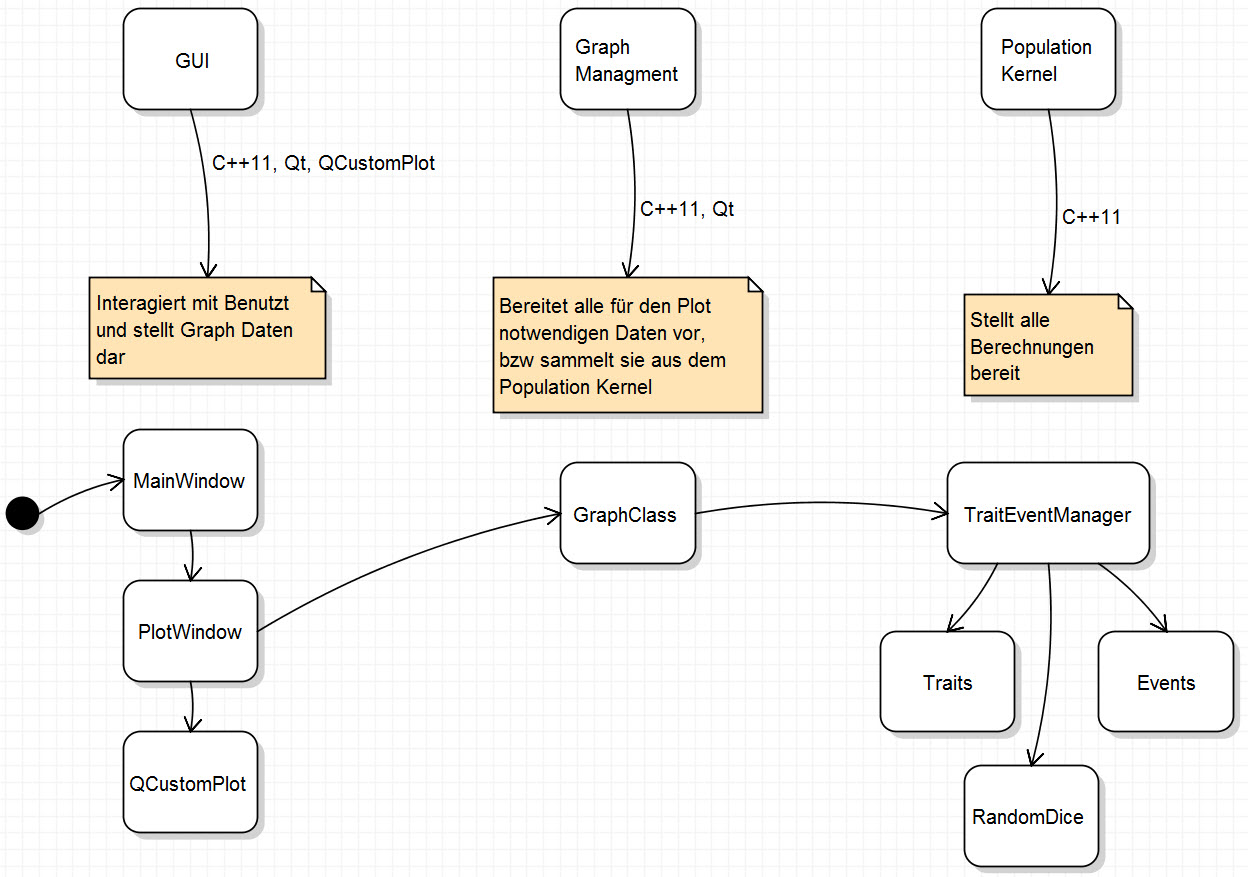
\includegraphics[width=0.7\linewidth]{./Pictures/Bild_Module}
		\caption[Module]{Arbeitsmodule und Klassenabhängigkeiten}
		\label{Module und Klassen}
	\end{figure}
	Innerhalb der Arbeitsschritte sollte dabei genau die selbe Regel der Unabhängigkeit gelten wie bei den Modulen.
	
	\subsection{Layout}
	\begin{itemize}
		\item Die Bedienung des Programms sollte das lesen und Anzeigen der Merkmals-Parameter bereitstellen. Da es viele Parameter gibt und die Anzahl der Parameter quadratisch mit der Anzahl der betrachteten Merkmale steigt, bietet sich das Lesen aus zuvor beschriebenen Dateien an.
		\begin{figure}[H]
			\centering
			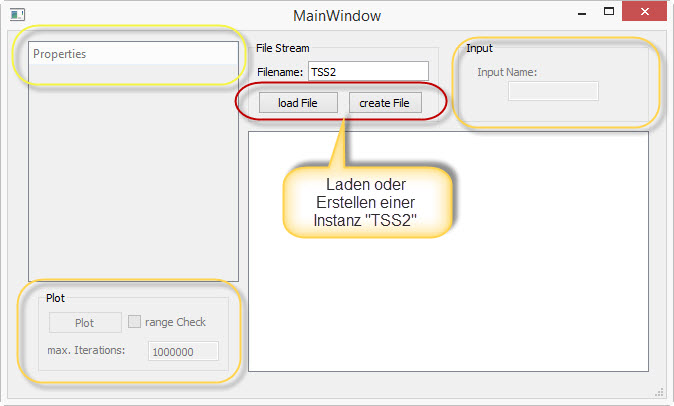
\includegraphics[width=0.7\linewidth]{./Pictures/MainWindow_Start}
			\caption[Startwindow]{MainWindow nach dem Start}
			\label{MainWindow_Start}
		\end{figure}

		Zur Darstellung der gelesenen Parameter habe ich ein Baumstruktur gewählt.
		\begin{figure}[H]
			\centering
			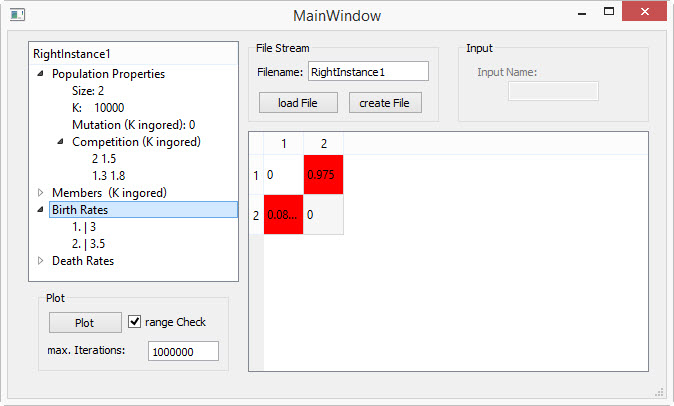
\includegraphics[width=0.7\linewidth]{./Pictures/MainWindow_ParameterBaum}
			\caption[MainWindow_Parameter]{MainWindow mit geladenen Parametern}
			\label{Baumstruktur}
		\end{figure}
		\item Die letzte Herausforderung bestand darin eine Instanz durch das Programm geleitet erstellen zu können. Während diese Aufgabe bei einer Konsolenanwendung (bekannt aus den klassischen c Programmen) denkbar einfach mit "{}printf"{} und "{}scanf"{} erledigt werden konnte, sollte bei einem GUI eine Lösung her die Inputkonflikte verhindert und das Einlesen der Daten denkbar einfach macht. Dafür war es sinnvoll "{}Enter"{} als Bestätigung abzufangen und sicherzustellen dass der Curser nur innerhalb des gewünschten Feldes bleibt.
		\begin{figure}[H]
			\centering
			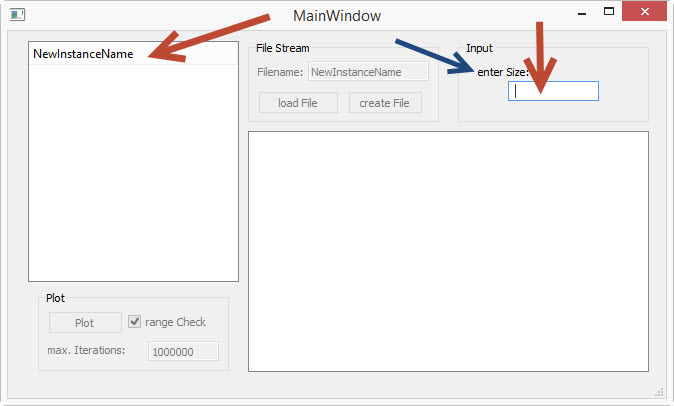
\includegraphics[width=0.7\linewidth]{./Pictures/MainWindow_createFile}
			\caption[erstelle Datei]{Nach Klick auf "{}create File"{} werden die neuen Parameter einzeln abgefragt}
			\label{fig:MainWindow_createFile}
		\end{figure}
		\begin{figure}[H]
			\centering
			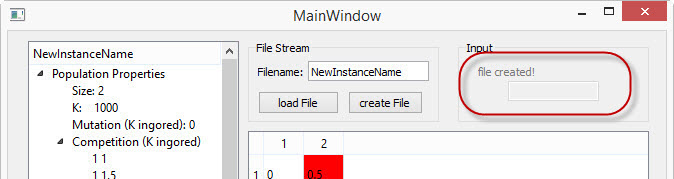
\includegraphics[width=0.7\linewidth]{./Pictures/MainWindow_FileCreated}
			\caption[Datei erstellt]{Nach Eingabe des letzten Parameters}
			\label{fig:MainWindow_FileCreated}
		\end{figure}
	\end{itemize}
	Was die Darstellung der Graphen angeht, hat sich ein einfaches Bild des fertigen Plots durchgesetzt, wobei das Zoomen und ziehen des Bildes notwendige Elemente zur Untersuchung des Graphen sind. Zusätzlich ist es notwendig viele Bilder vergleichen zu können. Hierfür wurde das Abspeichern des Bildes gewünscht.\\
	Die Simulation wird gestartet nachdem man auf den "{}Plot"{} Button drückt. Dabei wird ein neues Fenster geöffnet.
	\begin{figure}[H]
		\centering
		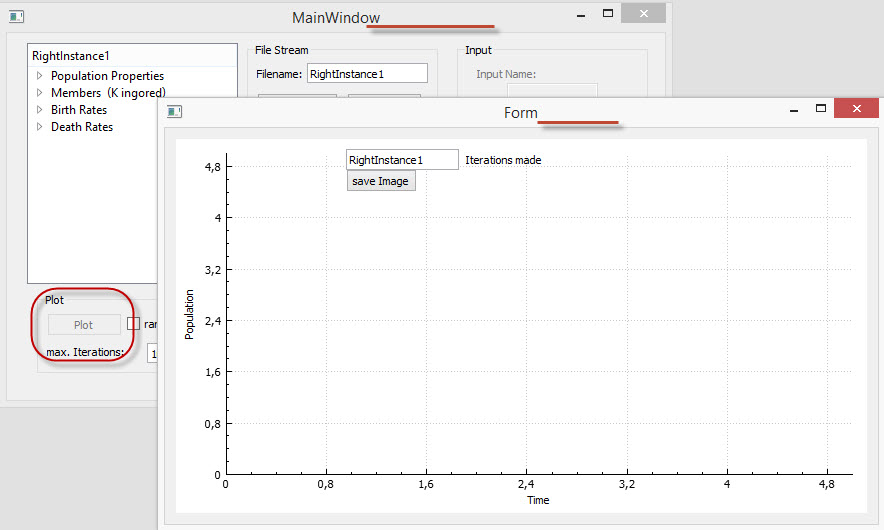
\includegraphics[width=0.7\linewidth]{./Pictures/PlotWindow_start}
		\caption[PlotWindow_start]{Start des PlotWindow}
		\label{PlotWindow_start}
	\end{figure}
	Sobald der Plot Button gedrückt wurde und das Fenster angezeigt wird, arbeitet die Simulation bereits im Hintergrund in einem eigenen Thread. Dort werden alle notwendigen Iterationen bzw. Sprünge der Population durchgeführt ohne den Hauptthread damit zu belasten.\\ Während dieser Arbeiterthread aktiv arbeitet wird der "{}Plot"{} Button ausgegraut um mehrfaches Auslösen zu vermeiden und um anzuzeigen dass die Rechnung im Gange ist.\\
	Der Arbeiterthread gewährleistet nicht nur eine flüssige Interaktion mit dem Programm, sondern verhindert auch effektiv dass das Betriebssystem denkt das Programm wäre Abgestürzt oder würde nicht mehr ordnungsgemäß funktionieren. Das würde sonst folgendes evtl. bekannte Bild hervorrufen:
	\begin{figure}[H]
		\centering
		
\includegraphics[width=0.7\linewidth]{./Pictures/KeineRueckmeldung}
		\caption[Keine Rueckmeldung]{Hauptthread wurde überlastet}
		\label{Keine Rueckmeldung}
	\end{figure}
	Wenn die Simulation  einen gewünschten Zustand erreicht hat, oder die maximale Anzahl an gewünschten Iterationen absolviert hat, werden anschließend maximal 10mio Punkte auf dem Koordinatensystem zu Graphen verbunden. Das kann so aussehen:
	\begin{figure}[H]
		\centering
		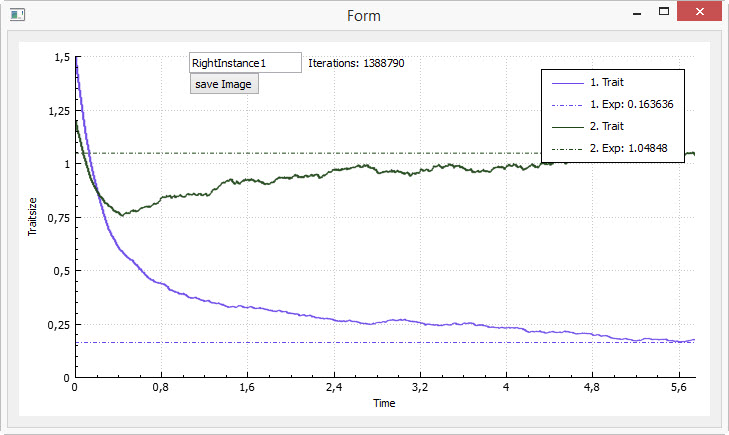
\includegraphics[width=0.7\linewidth]{./Pictures/PlotWindow_smallBPDL}
		\caption[PlotWindow]{PlotWindow mit Dimorpher Population}
		\label{PlotWindow}
	\end{figure}

\clearpage
\section{Verhaltenstest - Korrektheit der Implementation}
(Korrektheit des Algorithmus nicht notwendig bzw möglich)
Ein ganz besonders interessantes Thema ist die Korrektheit der Implementation. Diese ist generell mit steigender Komplexität schwerer zu prüfen (besonders bei Zufallsbedingten Simulationen).\\
Daher habe ich das Prinzip der "{}Testgetriebene Entwicklung"{}  (Test Driven Develeopment) verwendet.\\
Dabei werden Funktionen des Programms unter vorher festgelegten Bedingungen laufen gelassen und mit einem erwarteten Verhalten verglichen. Das Ergebnis ist eine Ausgabe für Erfolg oder Misserfolg des Tests. Folgend ein Beispiel für eine Implementation eines einfachen Tests der prüft ob alle Parameter korrekt aus der Datei in die Objekte geschrieben werden.
\begin{figure}[H]
	\centering
	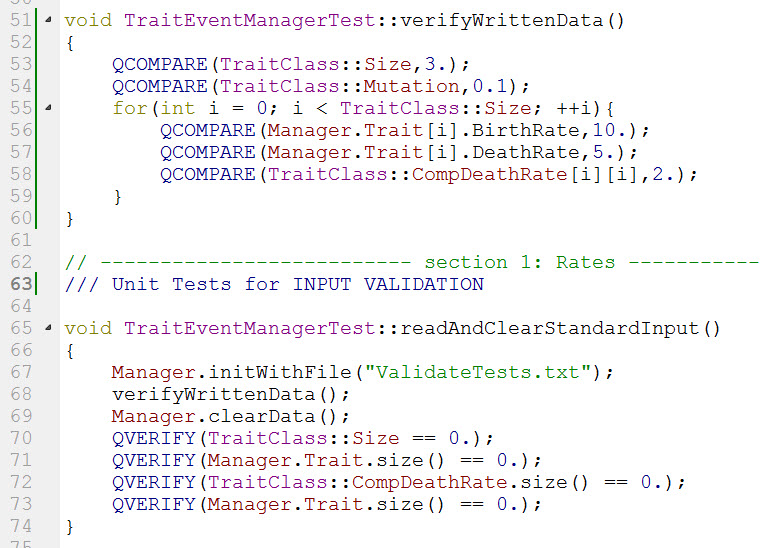
\includegraphics[width=0.7\linewidth]{./Pictures/UnitTest}
	\caption[UnitTest]{UnitTest versichert korrektes lesen von Parametern aus Datei}
	\label{Unit Test}
\end{figure}
Anschließend ein Beispiel für einen Durchlauf der Testfunktionen:
\begin{figure}[H]
	\centering
	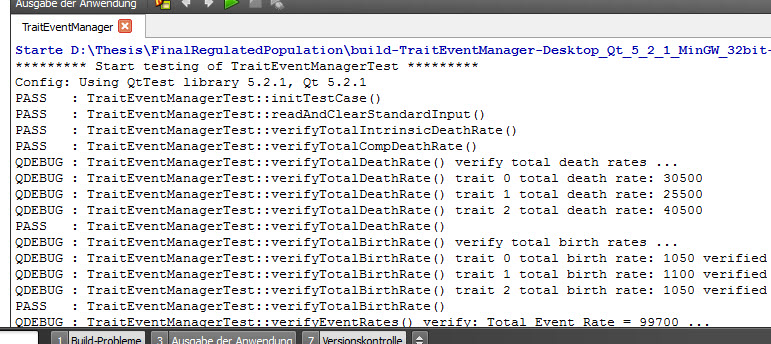
\includegraphics[width=0.7\linewidth]{./Pictures/TestResult_start}
	\caption[Test Resultat einer Test Datei]{Ergebnisse einiger Tests}
	\label{Test Results}
\end{figure}
Die Testfunktionen zeigen auch dass eine komplexe Verwendung der Simulationen über die graphische Darstellung hinaus einfach realisierbar ist.

	\subsection{Unit Tests der Algorithmusmodule}

\clearpage
\section{TSS Prozesse}
Bei TSS Prozessen beobachten wir wie sich Merkmale gegeneinander durchsetzten und sich verdrängen. (Tafelbild)\\
Genau wie bei der LPA-Normalisierung ergeben sich TSS-Prozesse(Trait Substitution Sequence) als Grenzprozesse von BPDL-Prozessen. Zu der LPA-Normalisierung sollten jedoch mit größer werdendem K die Mutationen seltener werden ($ \frac{1}{e^{VK}} << \mu_K << \frac{1}{K log(K)} $) , also die Mutationswahrscheinlichkeit gegen 0 streben. Skaliert man nun noch zusätzlich die Zeit, so führt dies dazu, dass die Zeit, die ein Merkmal benötigt, um sich gegenüber einem anderen durchzusetzen und dieses zu verdrängen, infinitesimal klein wird. Somit simulieren die TSS-Prozesse eine Population, die zu jedem Zeitpunkt monomorph ist und sich im entsprechenden (für $ K < \infty $ angepassten) Equilibrium befindet.\\
Spätestens jetzt wird die Fitness-Funktion interessant:
\[ f(x,y) = b(x) - d(x) - c(x,y)\bar{n}_y \]
Diese Fitness-Funktion gibt an, wie gut sich ein Merkmal gegenüber einem anderen durchsetzen kann. Sie ist die asymptotische Wachstumsrate von y, wenn x sich im Gleichgewichtszustand $ \bar{n}_x $ befindet und nur wenige Individuen von Typ y in der Population vorhanden sind. In der Simulation sieht man die Fitness der Merkmale zueinander in einer Matrix nach dem Laden der Parameter.
\begin{figure}[H]
	\centering
	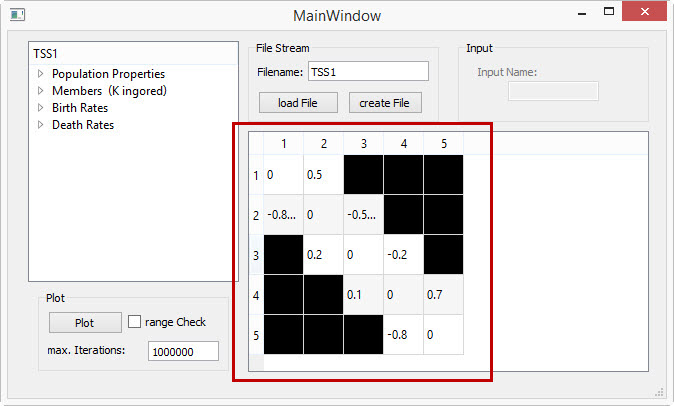
\includegraphics[width=0.7\linewidth]{./Pictures/MainWindow_BandMatrix}
	\caption[Fitness Matrix]{Fitness Bandmatrix}
	\label{MainWindow mit Fitness Bandmatrix}
\end{figure}
Mit der Fitness kann man eine Konvergenz der Wahrscheinlichkeit für das überleben einer Mutation vorhersagen:
\[ \frac{\left[ f(y,x)\right]_+ }{b(y)} \]
Da diese Wahrscheinlichkeit gerne bereits beim einlesen der Parameter angezeigt werden will, habe ich vor sie als farblich ansteigenden Akzent den Elementen der Zelle hinzuzufügen. Bisher wird in der Matrix etwas grün oder rot markiert. Rot falls eine Koexistenz vorliegt und grün wenn die Wahrscheinlichkeit für Dominanz des Mutanten über 50\% liegt.
\begin{figure}[H]
	\centering
	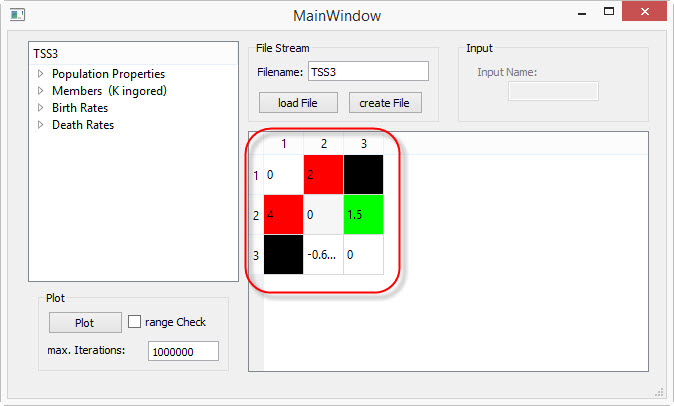
\includegraphics[width=0.7\linewidth]{./Pictures/MainWindow_red_green_loaded}
	\caption[MainWindow_redGreenFitness]{Fitness Matrix mit roten und gruenen akzenten}
	\label{fig:MainWindow_red_green_loaded}
\end{figure}
Wenn der einfache BPDL Simulator für die Simulation dieses Prozesses verwendet werden würde, würde durch die seltenen Mutationen
	
	\subsection{Algorithmus}
\clearpage
\section{Ausblick}

\begin{itemize}
	\item Weiteres Abbruchkriterium = Zeit : sehr einfach zu implementieren.
\end{itemize}

\clearpage
\bibliography{science1}

\clearpage

\section{Beweise}


\section{Fragen}
\begin{itemize}
	\item Normalisierung, Equilibrium und mono/dimorphe F"alle als einzelne Kapitel?
	\item Soll ich monomorphe BPDL Prozesse einf"uhren? Schlie"slich kann ich damit das fast sicheres Aussterben 
	\item Beweis der LPA-Normalisierung per Differentialgleichungen?
\end{itemize}

\section{Wozu hat es nicht mehr gereicht?}
Instanzbrowser oder Dateisuche.\\
einfaches Bearbeiten erstellter Instanzen.\\

\end{document}